\section{Numerical Experiments}
\label{experiments}
In this section, we present three sets of test cases to validate the derived formulations and implementations. The first case is a biaxial tension test which is often used to calibrate material constants. For isotropic materials, the analytical solution can be easily found if the material is assumed to be incompressible. The second case is the expansion of a $2$D cylinder. It is widely used to validate the numerical results because the theoretical solution can be found for some models. The last case is specific to biomechanics where the expansion of a $2$-layer artery vessel of a rabbit is examined.

\subsection{Biaxial Tension Test}
\label{biaxial_tension_test}
In this test, we examine the $3$ isotropic models (Neo-Hookean, Mooney-Rivlin, and Yeoh models) and $1$ anisotropic HGO model. Consider a long bar loaded equally in two directions with fixed tractions. The section of the bar is a $1$ $m^2$-square. As shown in Figure \ref{fig:biaxial_schematic}, the back surface is fixed in the $x$-direction; the left surface is fixed in the $y$-direction and the bottom surface is fixed in the $z$-direction. External tractions are applied to the front and right surfaces. 

\begin{figure}[H]
\centering
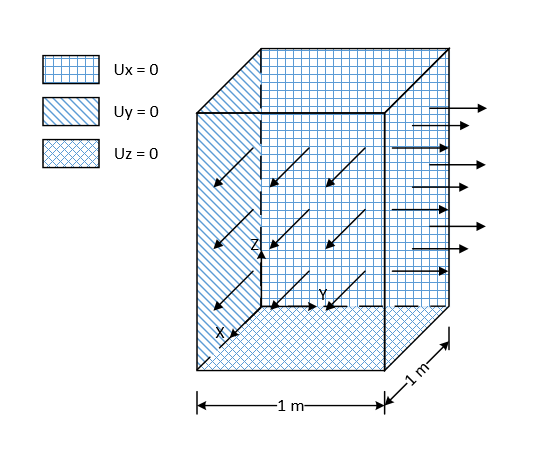
\includegraphics[width=.5\textwidth]{./figures/biaxial_schematic.png}
\caption{Schematic diagram of biaxial tension test}
\label{fig:biaxial_schematic}
\end{figure}

The bar is stretched by the tractions in $x$ and $y$ directions, and compressed in the $z$ direction in order to maintain the volume unchanged. The stretch $\lambda$ is defined as the ratio between the deformed length to the original length in $x$ and $y$ directions. For isotropic incompressible material the theoretical solution of the diagonal components of the PK2 stress is expressed as:
\begin{equation} \label{biaxialPK2}
S_{11} = S_{22} = 2(1 - {\lambda}^{-6})\left(\frac{\partial\Psi_\mathrm{iso}}{\partial\bar{I}_1} + {\lambda}^2\frac{\partial\Psi_\mathrm{iso}}{\partial\bar{I}_2}\right), \quad S_{33} = 0
\end{equation}
All the off-diagonal components are $0$.

Since the nonzero components of the PK2 stress are the same, we denote them as $S$. For Mooney-Rivlin model, plug Equation \ref{iso1} into \ref{biaxialPK2}, we have:

\begin{equation}
S = (1 - {\lambda}^{-6})(\mu_1 + \mu_2{\lambda}^2)
\end{equation}
Therefore, the nominal stress $P$ is:
\begin{equation}
P = \lambda S =  (\lambda - {\lambda}^{-5})(\mu_1 + \mu_2{\lambda}^2)
\end{equation}
When $\mu_2 = 0$ terms we have the nominal stress for Neo-Hookean model:
\begin{equation}
P = \lambda S =  \mu_1(\lambda - {\lambda}^{-5})
\end{equation}
Similarly, for Yeoh model:
\begin{equation}
P = \lambda S = 2(\lambda - {\lambda}^{-5})\left[c_1 + 2c_2(2{\lambda}^2 + {\lambda}^{-4} - 3) + 3c_3(2{\lambda}^2 + {\lambda}^{-4} - 3)^2\right]
\end{equation}



Table \ref{parameters} lists the material constants used in the isotropic models, which are curve-fitted from the standard ASTM412 tensile test results of the rubber used in the transmission mounts \cite{Sharma}. The Poisson's ratios for all the models are set to $\nu = 0.49999$, close enough to incompressibility.

\begin{table}[H]
\centering
\caption{Material Parameters of the Isotropic Models}
\begin{tabular} { l  l  l }
	\hline
	Neo-Hookean & Mooney-Rivlin & Yeoh \\
	\hline
	$\mu_1 = 0.595522$ MPa & $\mu_1 = 0.595522$ MPa & $c_1 = 0.358756$ MPa \\
	& $\mu_2 = 0.050381$ MPa & $c_2 = - 0.0508009$ MPa \\
	& & $c_3 = 0.0142132$ MPa \\
	\hline
	For all models, $\kappa = 1 \times 10^5 $ MPa \\
	\hline
\end{tabular}
\label{parameters}
\end{table}

Figure \ref{fig:biaxial1} shows the results of the theoretical calculations and numerical computations for all $3$ isotropic models for $\lambda$ in the range of $1$ to $1.8$. Since the traction is fixed in the original configuration, the nominal stress equals the traction. Perfect agreement is achieved at every discrete data point. As expected, in the small strain range, all these models have similar linear performance. It can be seen that $\mu_2$ in Mooney-Rivlin model acts as a modification to $\mu_1$ in Neo-Hookean model which increases the stiffness. In large strain range, the stiffness of Yeoh model grows quickly, becoming significantly larger than the others due to the inclusion of the higher order terms.


\begin{figure}[H]
	\centering
	\begin{subfigure}[b]{0.45\textwidth}
		\centering
		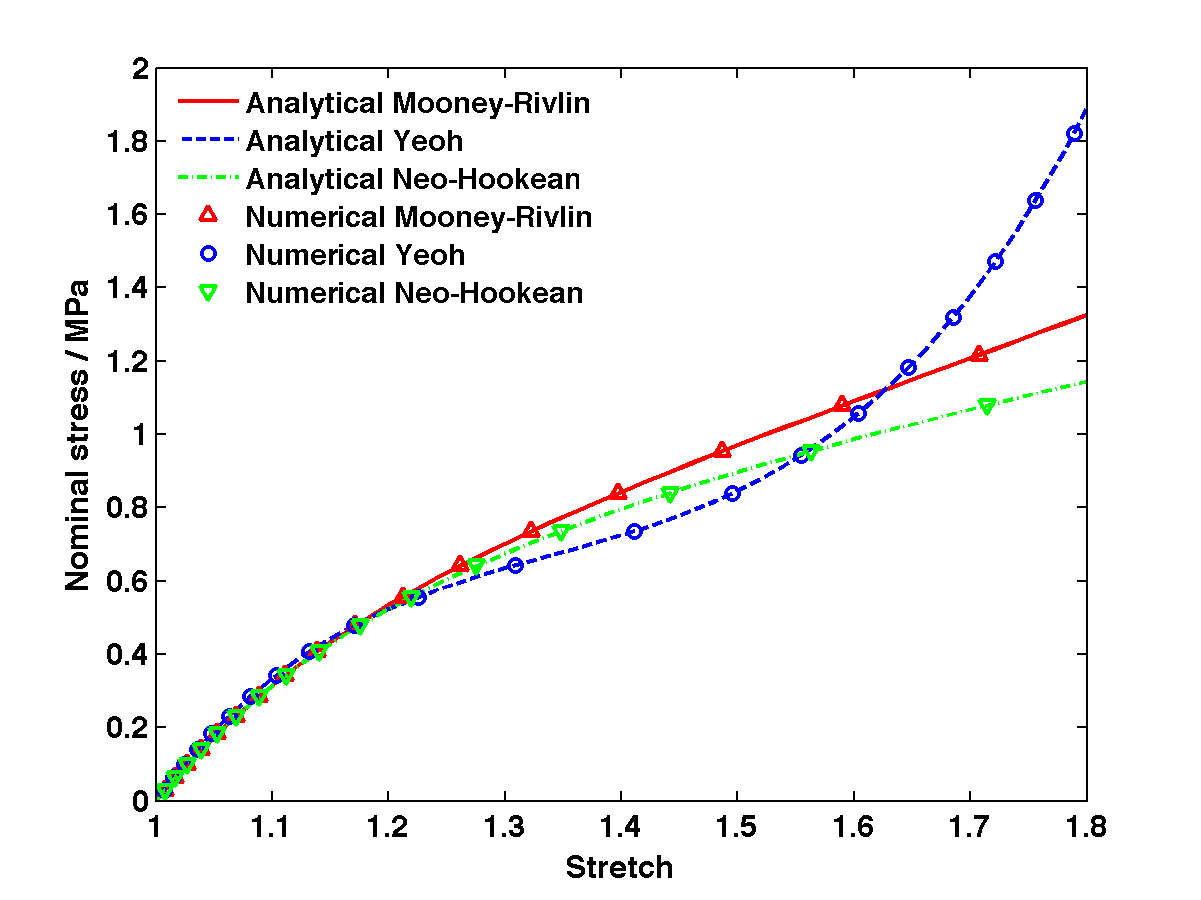
\includegraphics[width=\textwidth]{./figures/biaxial1.png}
		\caption{Isotropic models}
		\label{fig:biaxial1}
	\end{subfigure}
	\begin{subfigure}[b]{0.45\textwidth}
		\centering
		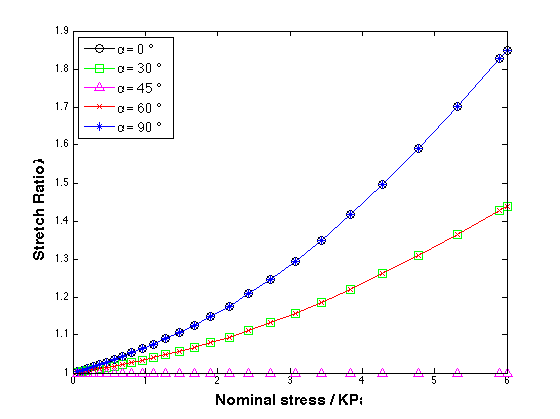
\includegraphics[width=\textwidth]{./figures/biaxial2.png}
		\caption{HGO model}
		\label{fig:biaxial2}
	\end{subfigure}
	\caption{Relationship of nominal stress to stretch in biaxial tension test}
\end{figure}


To demonstrate the anisotropy of HGO model, we compare the stretches in two directions in the biaxial tension test. We use the material parameters calibrated from the media layer of the artery in \cite{Holzapfel2} but only one direction is strengthened. That is, both two families of fibers are arranged in the same direction while the tractions are still applied in two directions. The material parameters are $\mu_1 = 3$ KPa, $k_1 = 2.3632$ KPa, $k_2 = 0.8393$ and $\kappa = 1 \times 10^5$ KPa. We vary the direction of the fibers measured by the angle from the $x$ direction denoted as $\alpha$, from $0^\circ$ to $90^\circ$ to observe the trends qualitatively as there exists no theoretical solution to it. 

The stretch ratio $\lambda$ is defined as $\lambda = 
\begin{cases}
	\lambda_y/\lambda_x, & \text{$\alpha = 0^\circ$, $30^\circ$ or $45^\circ$} \\
	\lambda_x/\lambda_y, & \text{$\alpha = 60^\circ$ or $90^\circ$}
\end{cases}
$ 
and Figure \ref{fig:biaxial2} shows the nominal stress, which is nothing but the traction applied to each surface, as a function of stretch ratio. As expected, the stretch ratio at $\alpha = 0^\circ$ is the same as $\alpha = 90^\circ$. These complementary angles of $\alpha$ yields the most asymmetric results since the stretch ratio is the largest for a given nominal stress. Same stretch ratios are obtained for $\alpha = 30^\circ$ and $\alpha = 60^\circ$. 
$\lambda_y$ is greater than $\lambda_x$ when $0^\circ < \alpha < 45^\circ$ since the $x$ direction is strengthened more. As the angle gets larger, $\lambda_x$ becomes greater too. When $\alpha = 45^\circ$ two directions become symmetric and the stretch ratio remains to be $1$.
 

\subsection{Cylindrical Pressure Vessel with Isotropic Models}
\label{pressure_vessel}
In the second test, we consider a vessel under internal pressure. This case is more challenging than the previous one, especially in the Cartesian coordinates system since the deformation varies both in the radial and the circumferential directions. As shown in Figure \ref{fig:vessel_schematic}, the cylinder has an internal radius of $R_i = 7$ m and an external radius of $R_o = 18.625$ m. Only a quarter of vessel is considered with plain strain assumption. Symmetry conditions are applied to the two sides to simulate a complete cylinder. The material parameters for the isotropic models are the same as the previous example, listed in Table \ref{parameters}. 
\begin{figure}[H]
	\centering
	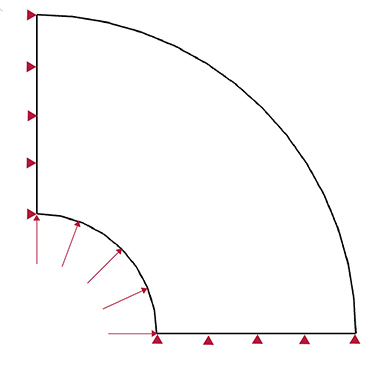
\includegraphics[width=0.3\textwidth]{./figures/vessel_schematic.jpg}
	\caption{Cross section of the vessel}
	\label{fig:vessel_schematic}
\end{figure}

As a benchmark, we model the vessel with Mooney-Rivlin model and compare the radial displacement, hoop stress, radial stress, and axial stress with the analytical solutions. For incompressible materials, the analytical solutions are found in \cite{Green} as follows: 
\begin{subequations}
\begin{align}
u_r &= -R + \sqrt{R^2 + b} \\
p &= - p_i - \mu_2 - (\mu_1 + \mu_2)\left(\log \frac{r}{R_i} + \frac{b}{2}(r^2 - {R_i}^2) - \log \frac{R}{R_i} + {\left(\frac{R_i}{r}\right)}^2 \right) \\
\sigma_{\theta\theta} &= p + \mu_2 + (\mu_1 + \mu_2)\left(\frac{r}{R}\right)^2 + C \\
\sigma_{rr} &= p + \mu_2 + (\mu_1 + \mu_2)\left(\frac{R}{r}\right)^2 + C \\
\sigma_{zz} &= p +  \mu_1 + \mu_2\left[\left(\frac{R}{r}\right)^2 + \left(\frac{r}{R}\right)^2\right] + C
\end{align}
where $R$ and $r$ are the radial coordinate before and after deformation, $p$ is the hydrostatic pressure, $u_r$ is the radial displacement, and $\sigma_{\theta\theta}$, $\sigma_{rr}$ and $\sigma_{zz}$ are the hoop, radial and axial stresses, respectively. $C$ is an arbitrary constant to determined by the reference pressure since the material is incompressible. $b$ is a constant determined by the internal pressure $p_i$ as:
\begin{align}
p_i &= 2(\mu_1 + \mu_2)\left(\log \frac{{R_i}^2 + b}{{R_o}^2 + b} - 2\log \frac{R_i}{R_o} +
b\frac{{R_o}^2 - {R_i}^2}{({R_o}^2+b)({R_i}^2+b)}\right)
\end{align}
\end{subequations} 

Figure \ref{fig:mooney-rivlin1} shows the stress components and the radial displacement along the radial direction under the pressure of $p_i = 200$ KPa. Good agreement is achieved on all the components. There are $21$ nodes that are uniformly distributed in the radial direction. As expected, point on the outer surface undergoes less radial displacement than the inner surface in order to keep the area of cross-section unchanged. All the components of the Cauchy stress exhibit nonuniform distribution. The absolute value of hoop stress and radial stress on the inner surface are more significant than the outer surface. This is not altered by the value of the material constants or the pressure. But by setting different material constants along the radial direction one can obtain more uniform stress distributions \cite{Batra}. Note that the axial stress is usually hard to validate and seldom shown in literature. The responses of a range of internal pressures are also studied. We pick the node at the midpoint in the radial direction ($R = 12.8125$ m) and study its deformation under different internal pressures from $50$ to $350$ KPa. As shown in Fig \ref{fig:mooney-rivlin2}, the computational result and analytical solution agree perfectly with each other. The variation of the radial displacement and the stress are nonlinear in the sense that the absolute value increases faster at greater pressure. This is similar to what we observed in Figure \ref{fig:biaxial1}.

\begin{figure}[H]
	\begin{subfigure}[b]{0.5\textwidth}
		\centering
		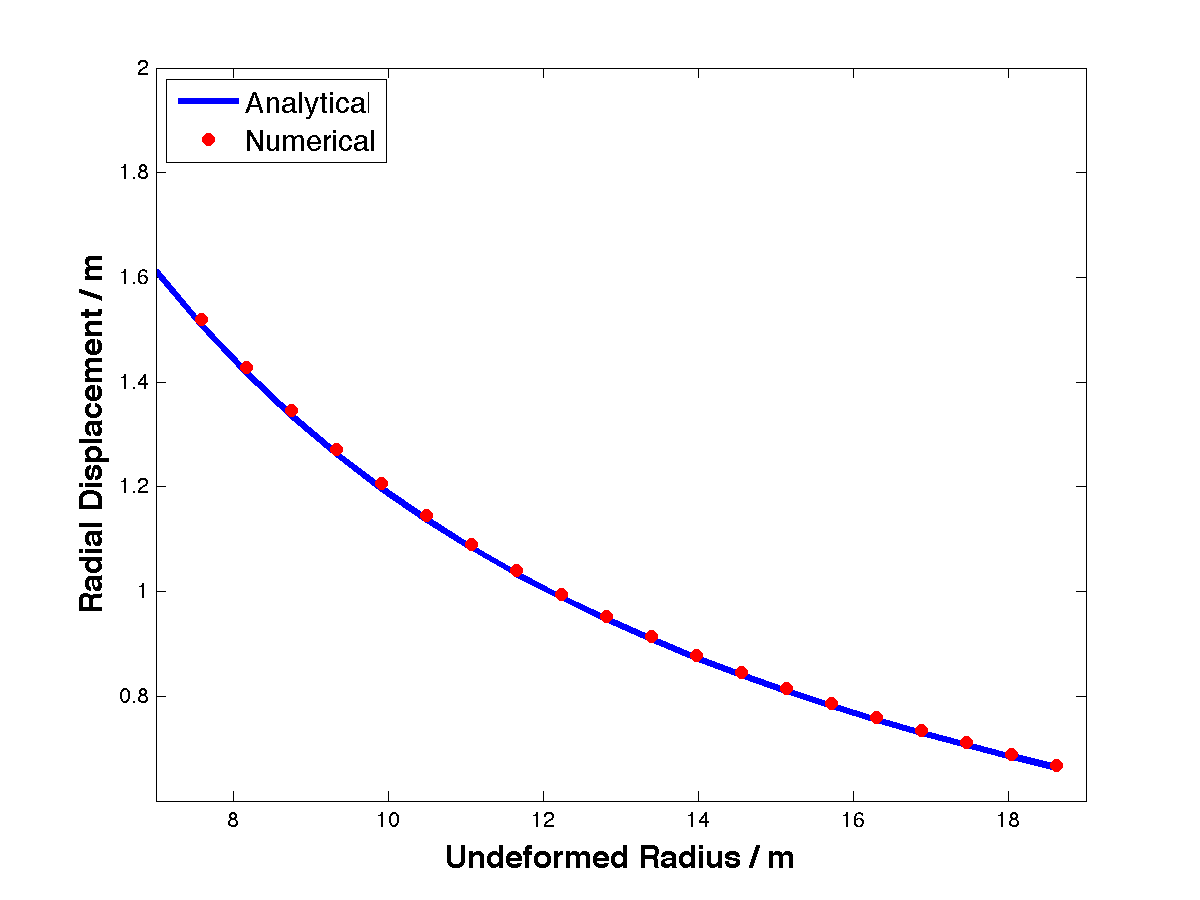
\includegraphics[width=\textwidth]{./figures/ur_200.png}
		\caption{Radial displacement}
		\label{ur_200}
	\end{subfigure}
	\begin{subfigure}[b]{0.5\textwidth}
		\centering
		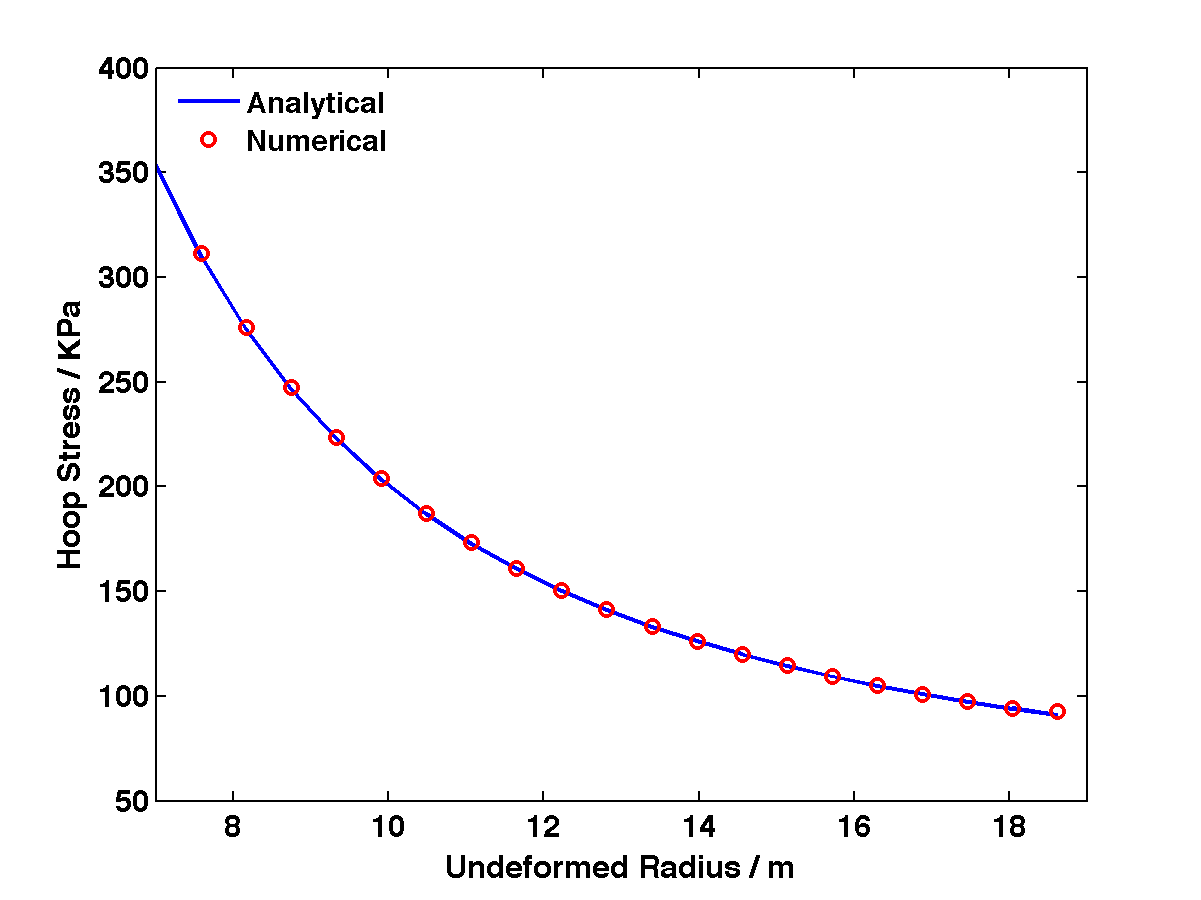
\includegraphics[width=\textwidth]{./figures/hoop_stress_200.png}
		\caption{Hoop stress}
		\label{hoop_200}
	\end{subfigure}
	
	\begin{subfigure}[b]{0.5\textwidth}
		\centering
		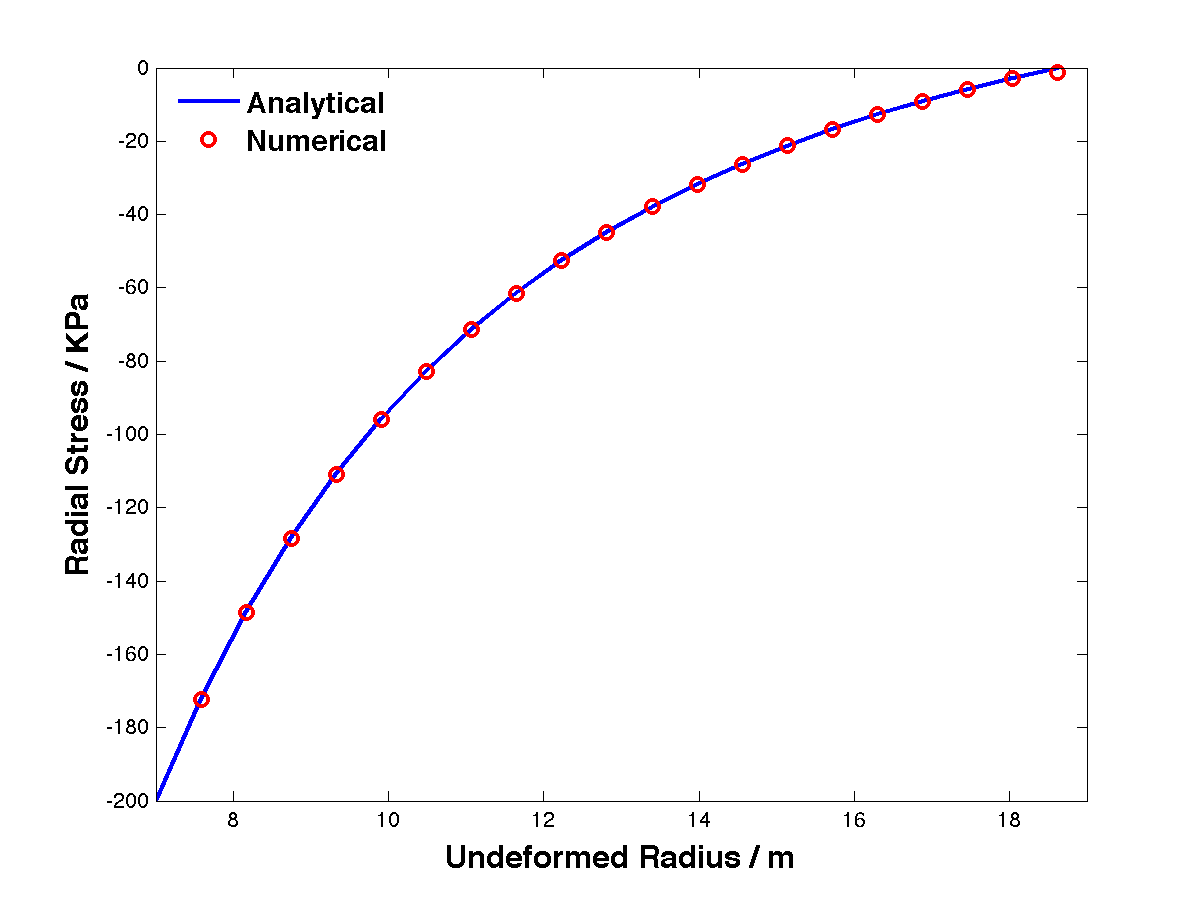
\includegraphics[width=\textwidth]{./figures/radial_stress_200.png}
		\caption{Radial stress}
		\label{radial_200}
	\end{subfigure}
	\begin{subfigure}[b]{0.5\textwidth}
		\centering
		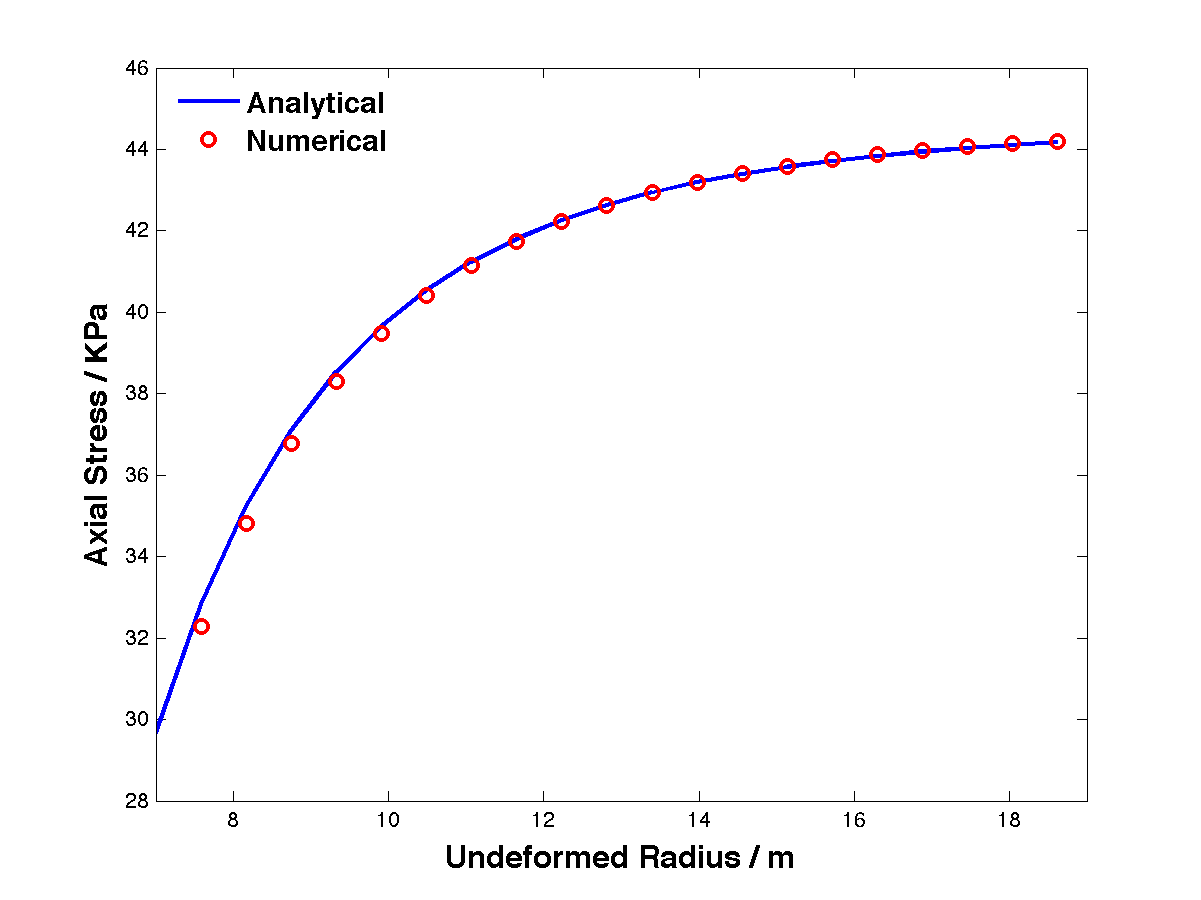
\includegraphics[width=\textwidth]{./figures/axial_stress_200.png}
		\caption{Axial stress}
		\label{axial_200}
	\end{subfigure}
	\caption{Vessel expansion under $p_i = 200$ KPa with Mooney-Rivlin model}
	\label{fig:mooney-rivlin1}
\end{figure}

\begin{figure}[H]
	\begin{subfigure}[b]{0.5\textwidth}
		\centering
		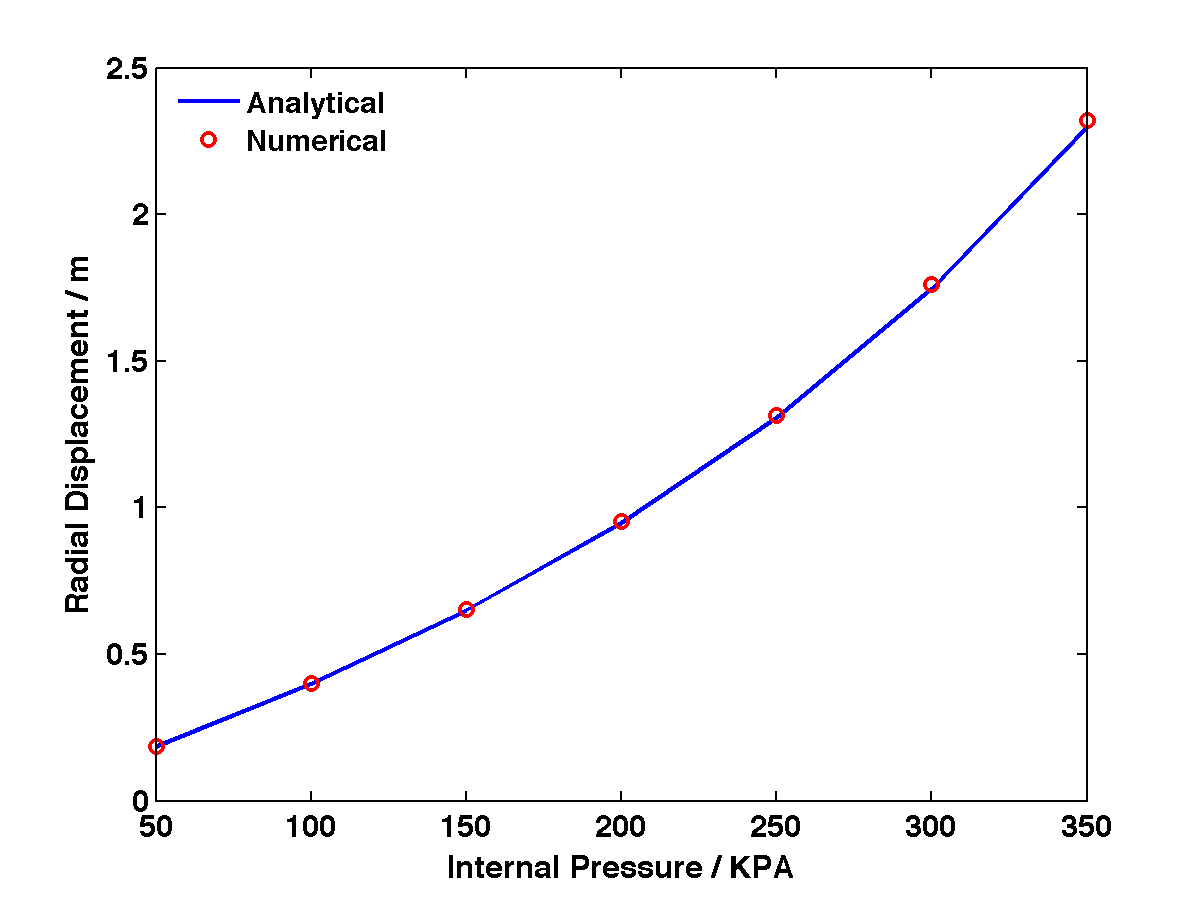
\includegraphics[width=\textwidth]{./figures/ur.png}
		\caption{Radial displacement}
		\label{ur}
	\end{subfigure}
	\begin{subfigure}[b]{0.5\textwidth}
		\centering
		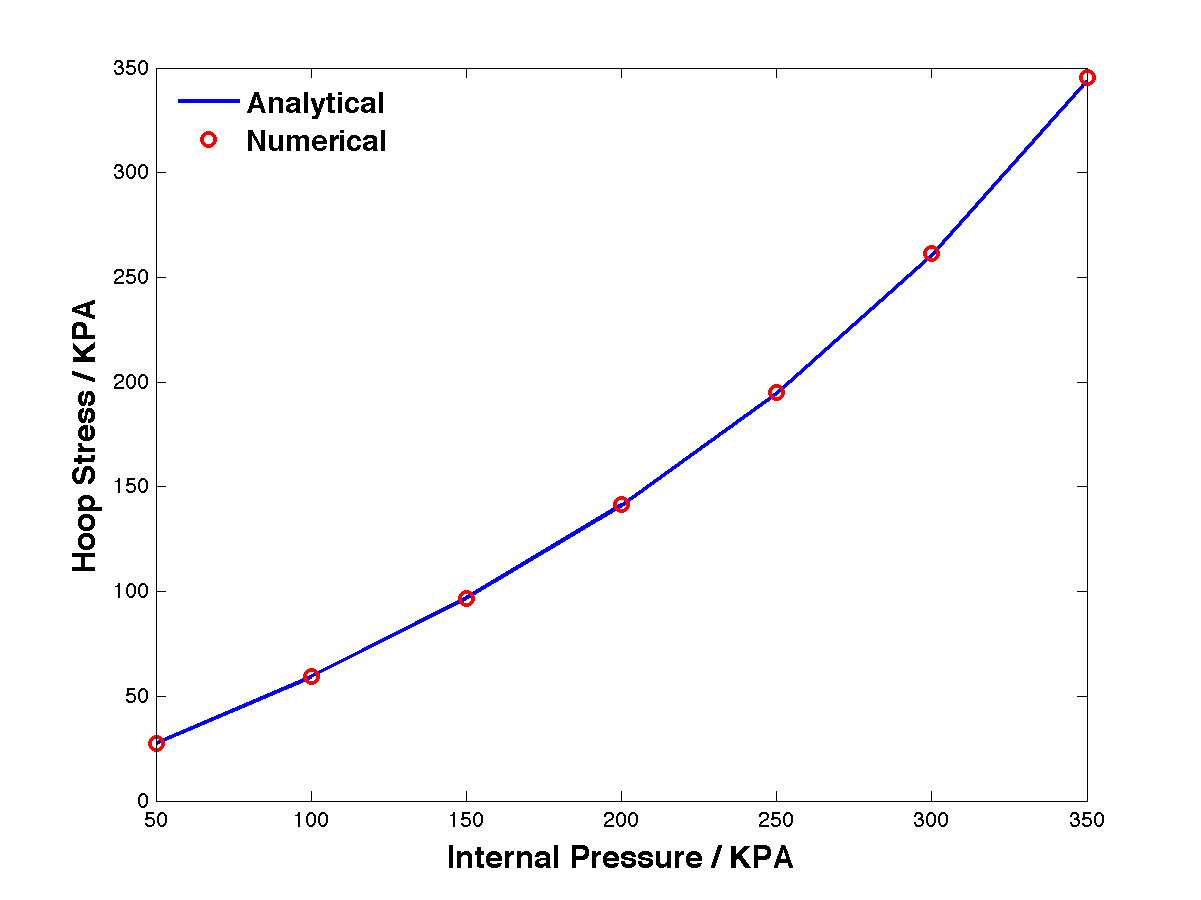
\includegraphics[width=\textwidth]{./figures/hoop.png}
		\caption{Hoop stress}
		\label{hoop}
	\end{subfigure}
	
	\begin{subfigure}[b]{0.5\textwidth}
		\centering
		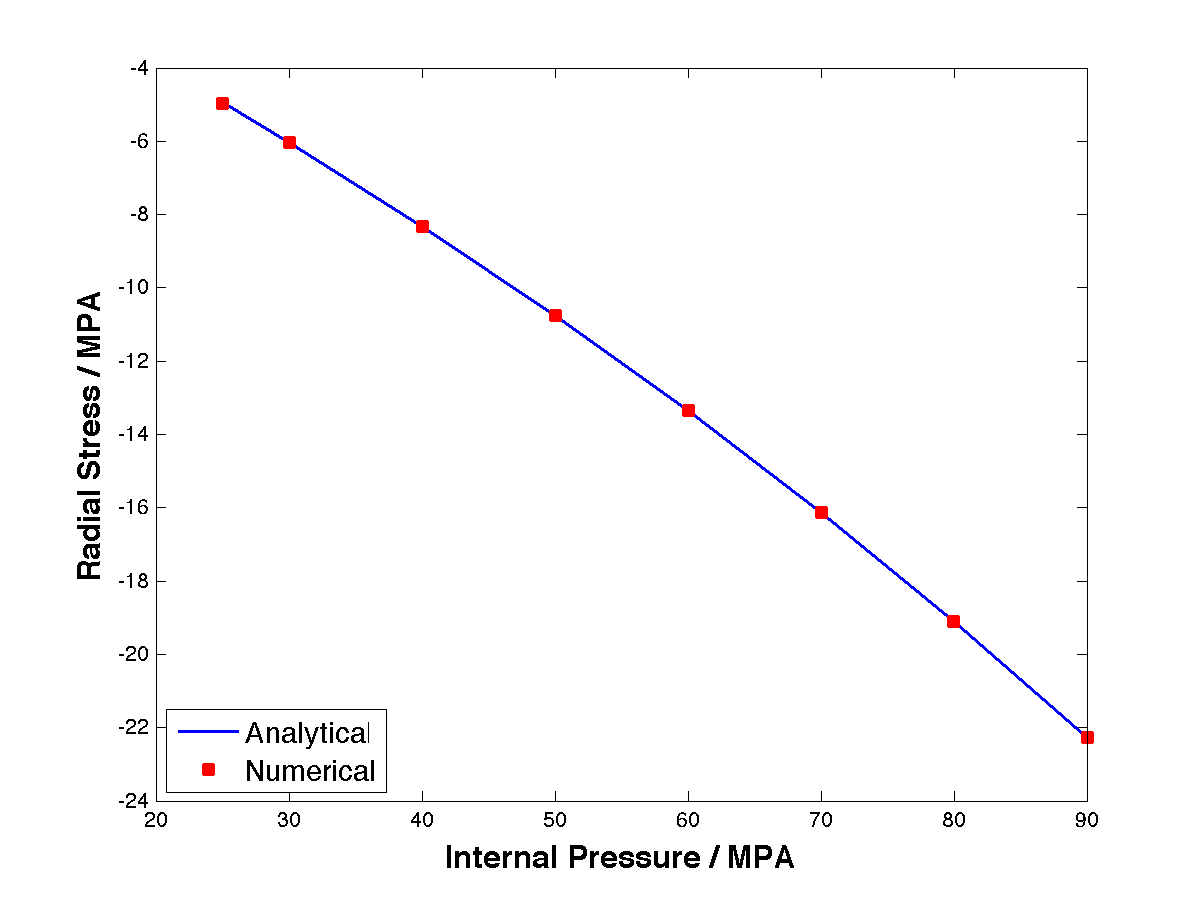
\includegraphics[width=\textwidth]{./figures/radial.png}
		\caption{Radial stress}
		\label{radial}
	\end{subfigure}
	\begin{subfigure}[b]{0.5\textwidth}
		\centering
		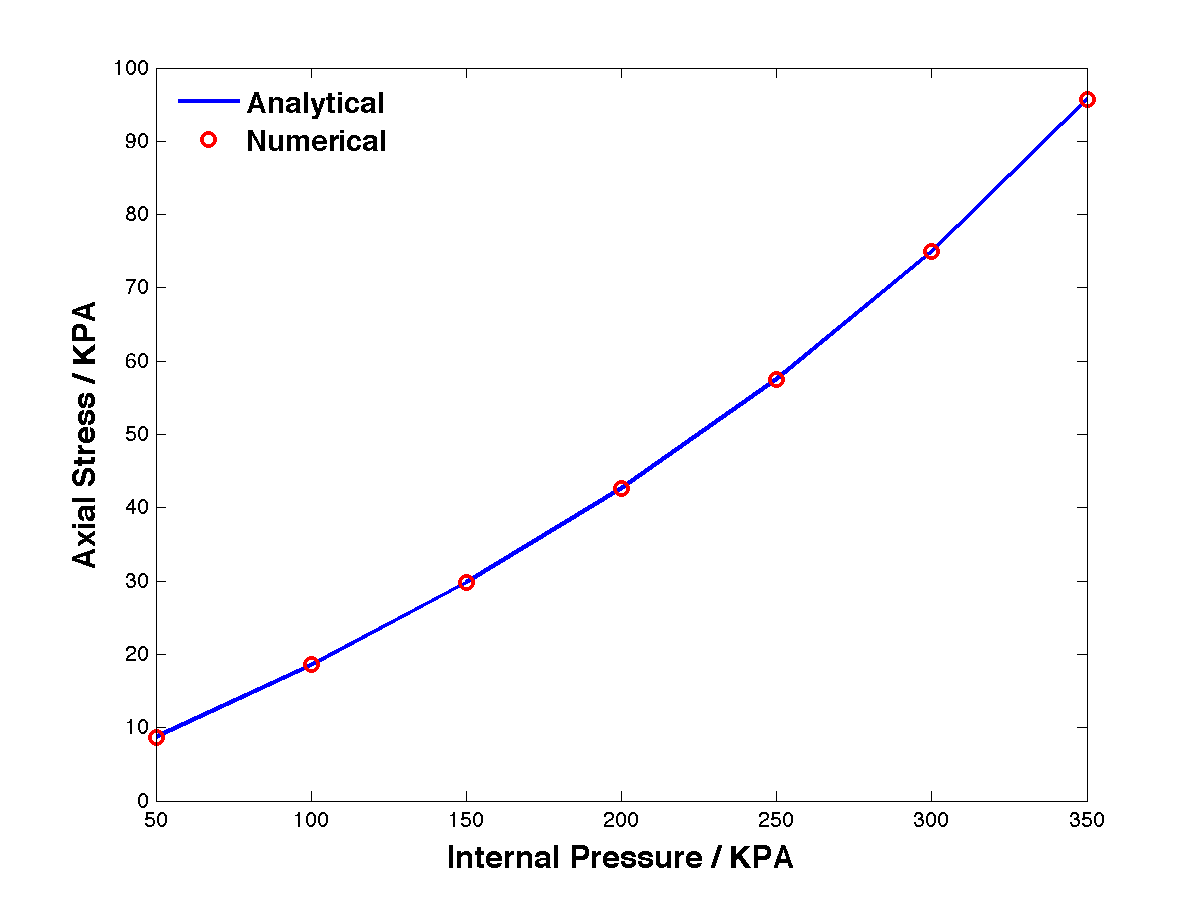
\includegraphics[width=\textwidth]{./figures/axial.png}
		\caption{Axial stress}
		\label{axial}
	\end{subfigure}
	\caption{Vessel expansion under different pressure with Mooney-Rivlin model}
	\label{fig:mooney-rivlin2}
\end{figure}

With the validated implementation of the Mooney-Rivlin model, we then compare the performance of Neo-Hookean, Mooney-Rivlin, and Yeoh model. Figure \ref{fig:models} shows the results of these models under an inner pressure of $p_i = 350$ KPa. All these isotropic models have similar trends, and the discrepancies among different models decrease from the inner surface to the outer surface. It implies that under a moderate pressure, different isotropic models do not make too much difference. The performance of the Yeoh model is very close to the Neo-Hookean model and stiffening effect does not occur. This is because they both have only one invariant and the strain is not large enough for Yeoh model to demonstrate its particular characteristics due to the higher order term. Considering in this case the maximum strain is already significant, and the expansion of vessels is not likely to exceed this maximum, it is expected that Yeoh model and Neo-Hookean model behave similarly.

\begin{figure}[H]
	\begin{subfigure}[b]{0.5\textwidth}
		\centering
		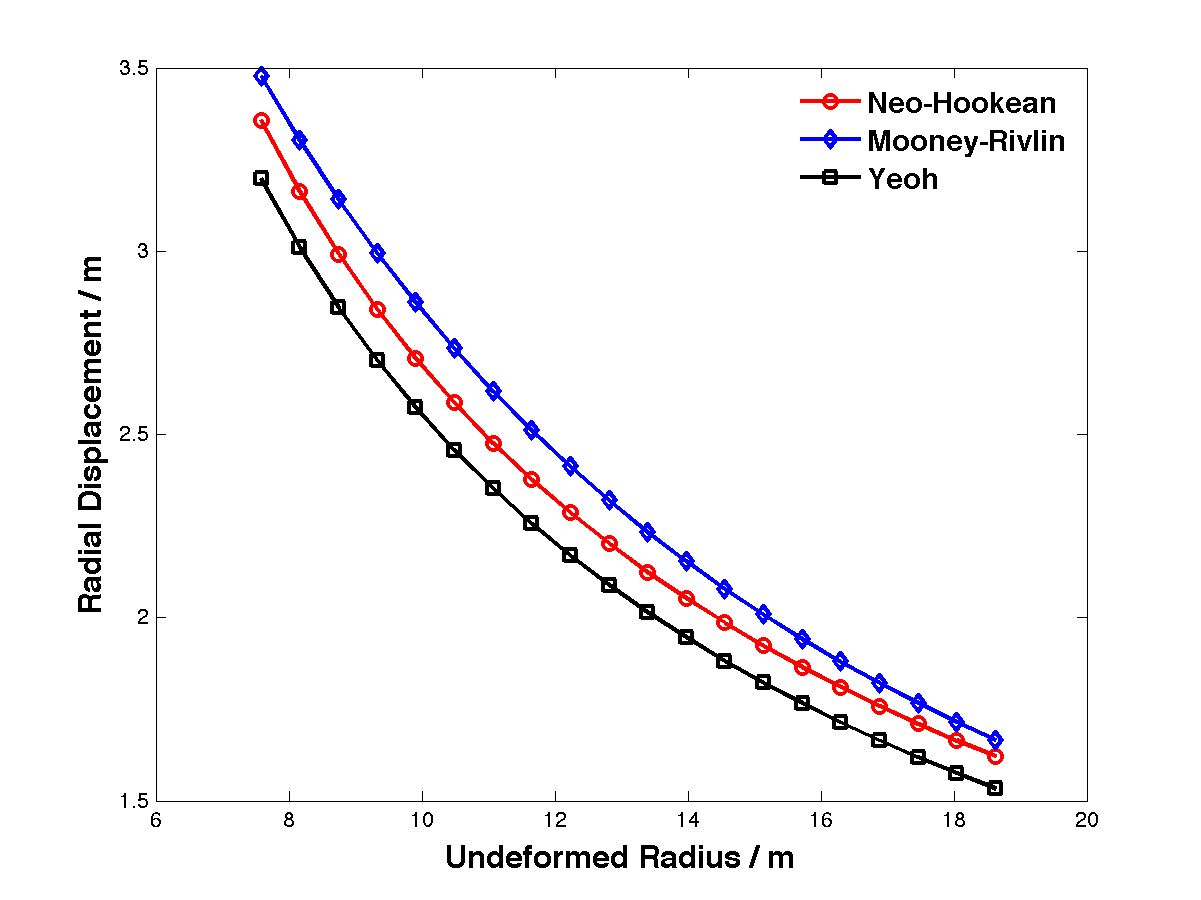
\includegraphics[width=\textwidth]{./figures/ur_models.png}
		\caption{Radial displacement}
		\label{ur_models}
	\end{subfigure}
	\begin{subfigure}[b]{0.5\textwidth}
		\centering
		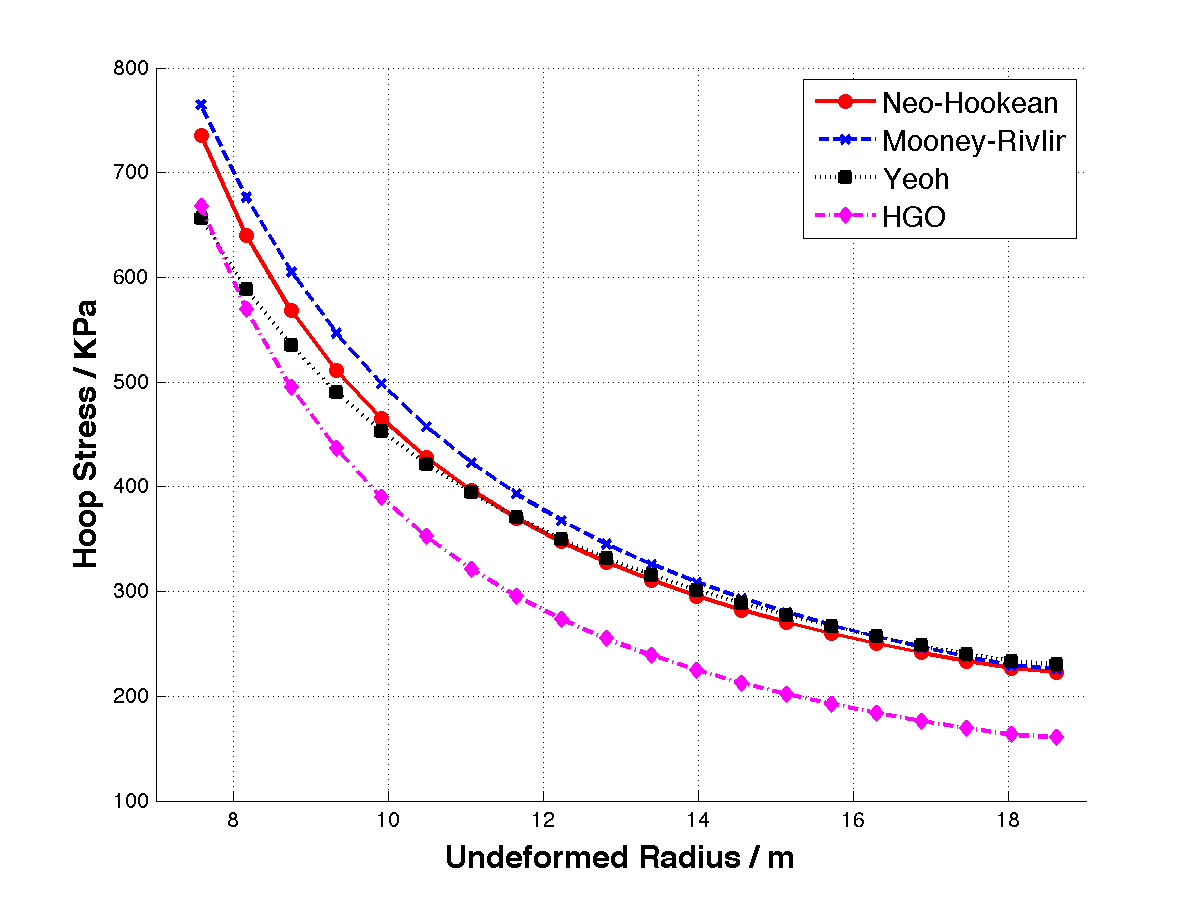
\includegraphics[width=\textwidth]{./figures/hoop_models.png}
		\caption{Hoop stress}
		\label{hoop_models}
	\end{subfigure}
	
	\begin{subfigure}[b]{0.5\textwidth}
		\centering
		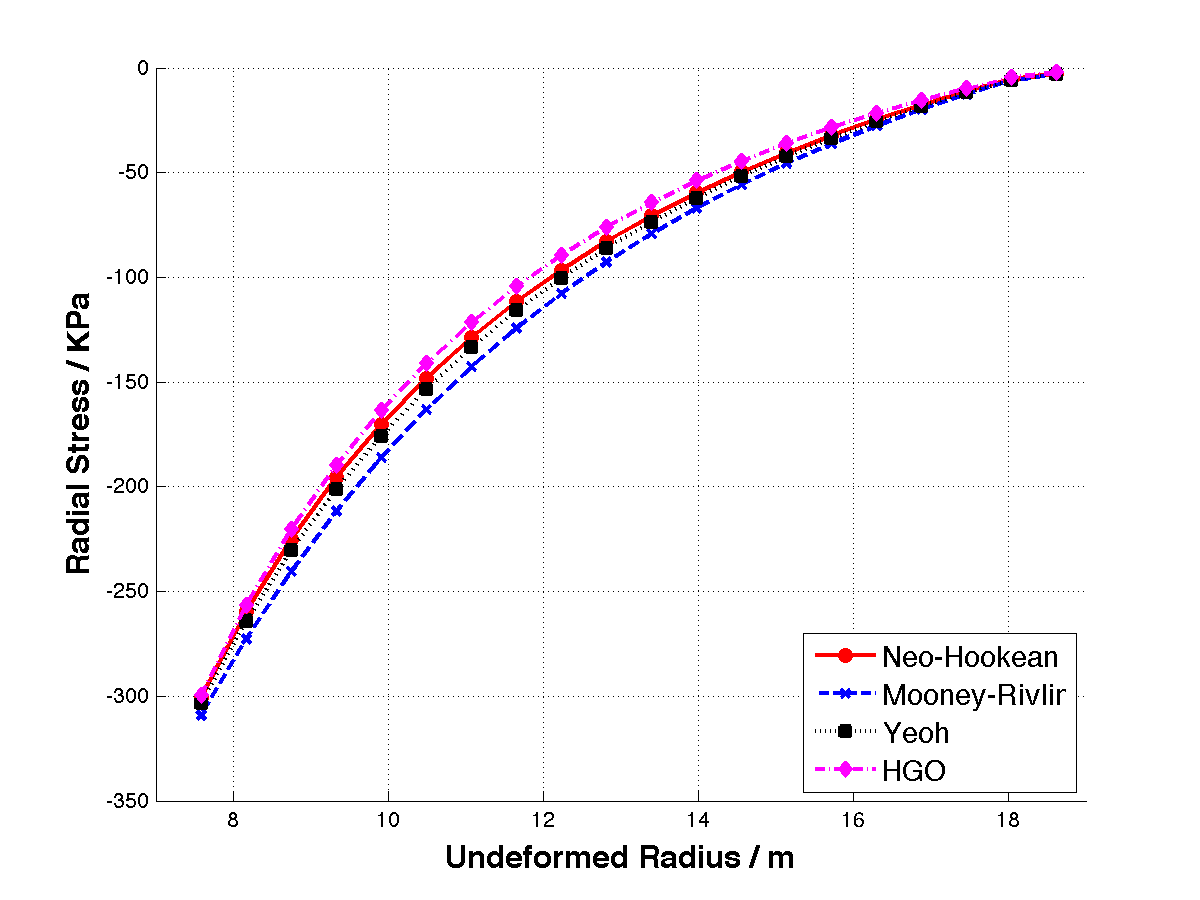
\includegraphics[width=\textwidth]{./figures/radial_models.png}
		\caption{Radial stress}
		\label{radial_models}
	\end{subfigure}
	\begin{subfigure}[b]{0.5\textwidth}
		\centering
		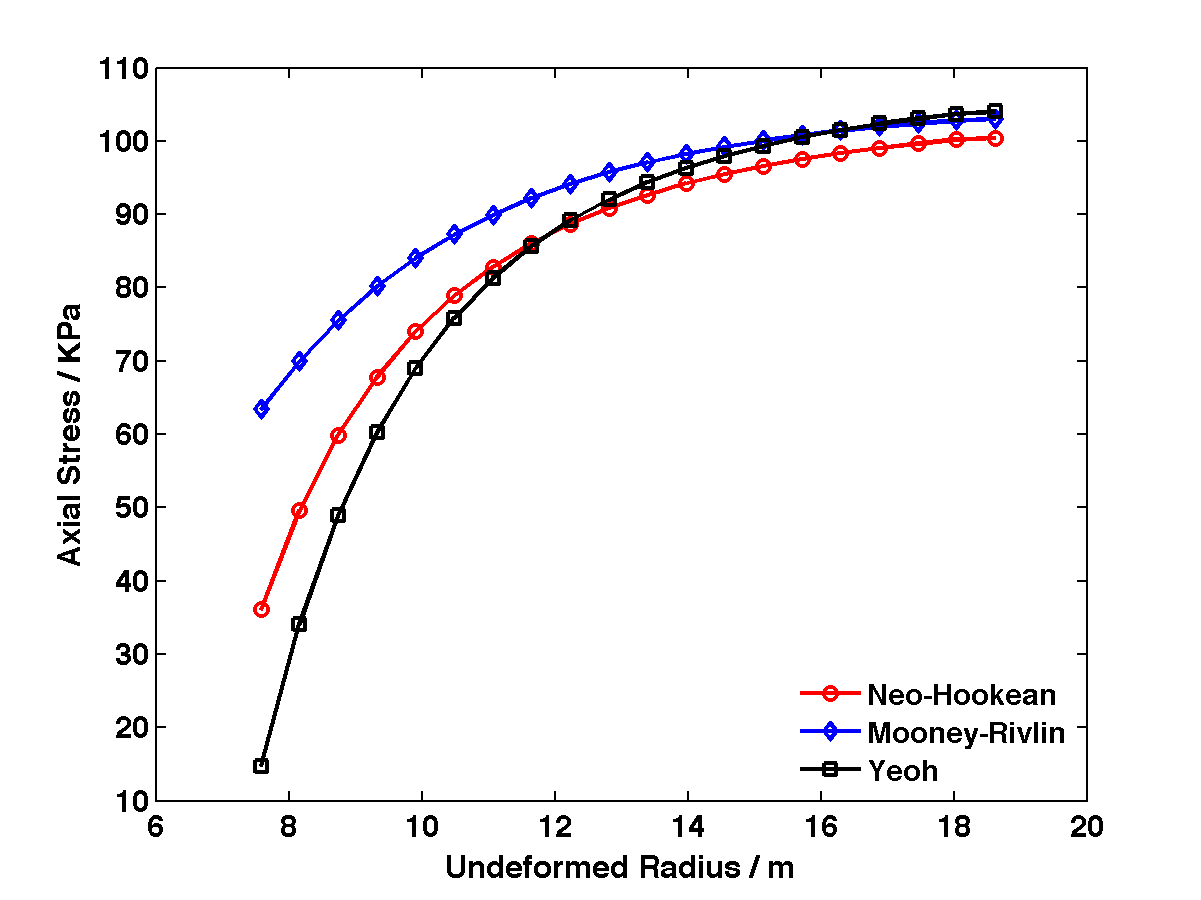
\includegraphics[width=\textwidth]{./figures/axial_models.png}
		\caption{Axial stress}
		\label{axial_models}
	\end{subfigure}
	\caption{Vessel expansion with different models under $350$ KPa}
	\label{fig:models}
\end{figure}

\subsection{Expansion of a $2$-layer Vessel}
In the last case, we use HGO model to simulate the expansion of the carotid artery of a healthy rabbit. The artery tissue is consist of three layers: intima, media, and adventitia. Here we only consider media and adventitia since the intima of young health vessels is made up of only one layer of endothelial cells and is insignificant in terms of mechanics. Research shows that the adventitia and the media have different mechanical properties \cite{Keitzer, Fung3}. The media is consist of a complex three-dimensional network of smooth muscle cells, elastin and collagen filbrils \cite{Holzapfel2}. According to \cite{Rhodin}, the media is reinforced by a number of concentrically fiber-reinforced medial layers. The adventitia is also reinforced by wavy collagen fibrils arranged in helical structures but is much less stiff than the media. Therefore the artery is modeled as $2$-layer cylindrical vessel with $\mu_1 = 3.0$ KPa, $k_1 = 2.3632$ KPa, $k_2 = 0.8393$ for the media layer and $\mu_1 = 0.3$ KPa, $k_1 = 0.5629$ KPa, $k_2 = 0.7112$ for the adventitia layer. The geometry of the artery is shown in Figure \ref{fig:vessel_schematic3}. The thickness of the media is $0.26$ mm, while the thickness of adventitia is $0.13$ mm. Two families of fibers are arranged in the $\theta-z$ plane, being symmetric about the $\theta$-direction. The angles between the fiber directions and the circumferential direction are denoted as $\pm\beta$. In the media, $\beta = 29.0^\circ$ and in the adventitia $\beta = 62.0^\circ$. The fibers induce the anisotropy but maintain the orthotropy. The geometry and material parameters, including the fiber directions we used are determined by Holzapfel \cite{Holzapfel2}, as shown in Table \ref{table:artery}. An internal pressure of $10$ KPa is applied. 

\begin{figure}[H]
\centering
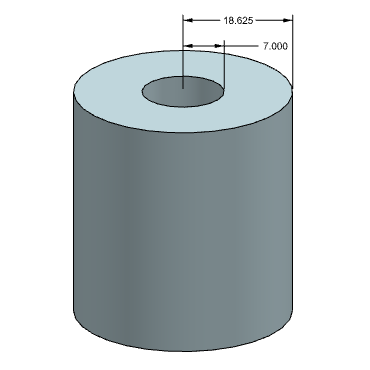
\includegraphics[width=.3\textwidth]{./figures/vessel_schematic2.png}
\caption{Schematic diagram for the artery model}
\label{fig:vessel_schematic3}
\end{figure}

\begin{table}[H]
\centering
\caption{The Configuration of the Artery Model}
\label{table:artery}
\begin{tabular}{ l l l l l l l}
\hline
& $\mu_1$(KPa) & $k_1$(KPa) & $k_2$(-) & $\kappa$(KPa) & $r$(mm) & $\beta(^\circ)$ \\
 \hline
 Media &   $3.0$ & $2.3632$ & $0.8393$ & $10^5$ & $[0.71, 0.97)$ & $29.0$\\
 Adventitia & $0.3$ & $0.5629$ & $0.7112$ & $10^5$ & [0.97, 1.1] & $62.0$\\
 \hline
\end{tabular}
\end{table}

The \emph{in vivo} artery is not stress-free even without lumen pressure, this initial stress is known as residual stress. The release of the residual stress results in a longitudinal and radial retraction \cite{Fung4, Holzapfel3}. Therefore in experiments and computations, a pre-stretch is often applied. Other than that, open angle method is also frequently used to account for the residual stress \cite{Kassab, Finet}. In this work we apply an axial pre-stretch of $\lambda = 1.7$ without open angle to the artery to examine the effect of the pre-stress. Figure \ref{fig:artery} shows the computational results of both the non-pre-stretched and pre-stretched artery, compared with the results obtained with COMSOL. 

The change in the displacement and stress distribution is obvious. With the pre-stretching, radial displacement drops significantly, but the decrease in the outer surface is much more. It means that the outer wall of the deformed vessel does not move much but the inner wall is squeezed drastically, absorbing most of the energy. The distribution of hoop stress and axial stress are more uneven with the pre-stretching and that of radial stress does not change a lot. With the pre-stretching, the hoop and axial stress are very high on the inner wall and taper off rapidly. Notice that the hoop stress and the axial stress have an steep drop at the intersection of two layers ($R = 0.97$ mm) while the radial stress is more smooth. Also the axial stress with pre-stretching shows a concave shape, and the minimum stress appears at the intersection. This effect is also found in the experiments presented in \cite{Keitzer}.

Our study agrees well with COMSOL, except for the minor differences at the intersection of two layers. The results of our code shows a more smooth transition at the intersection than COMSOL does. The reason is trivial: one must explicitly divide the mesh into two parts, generating a physical interface in order to assign different material parameters to two layers in COMSOL. While in our implementation the intersection is virtual, nothing more than a criterion to decide which set of material parameters to use. The vessel remains a whole part and there is no node lying on the intersection. If we refine the mesh solution at the intersection then a shaper change can be captured, approaching to the discontinuity shown in COMSOL.

\begin{figure}[H]
	\begin{subfigure}[b]{0.5\textwidth}
		\centering
		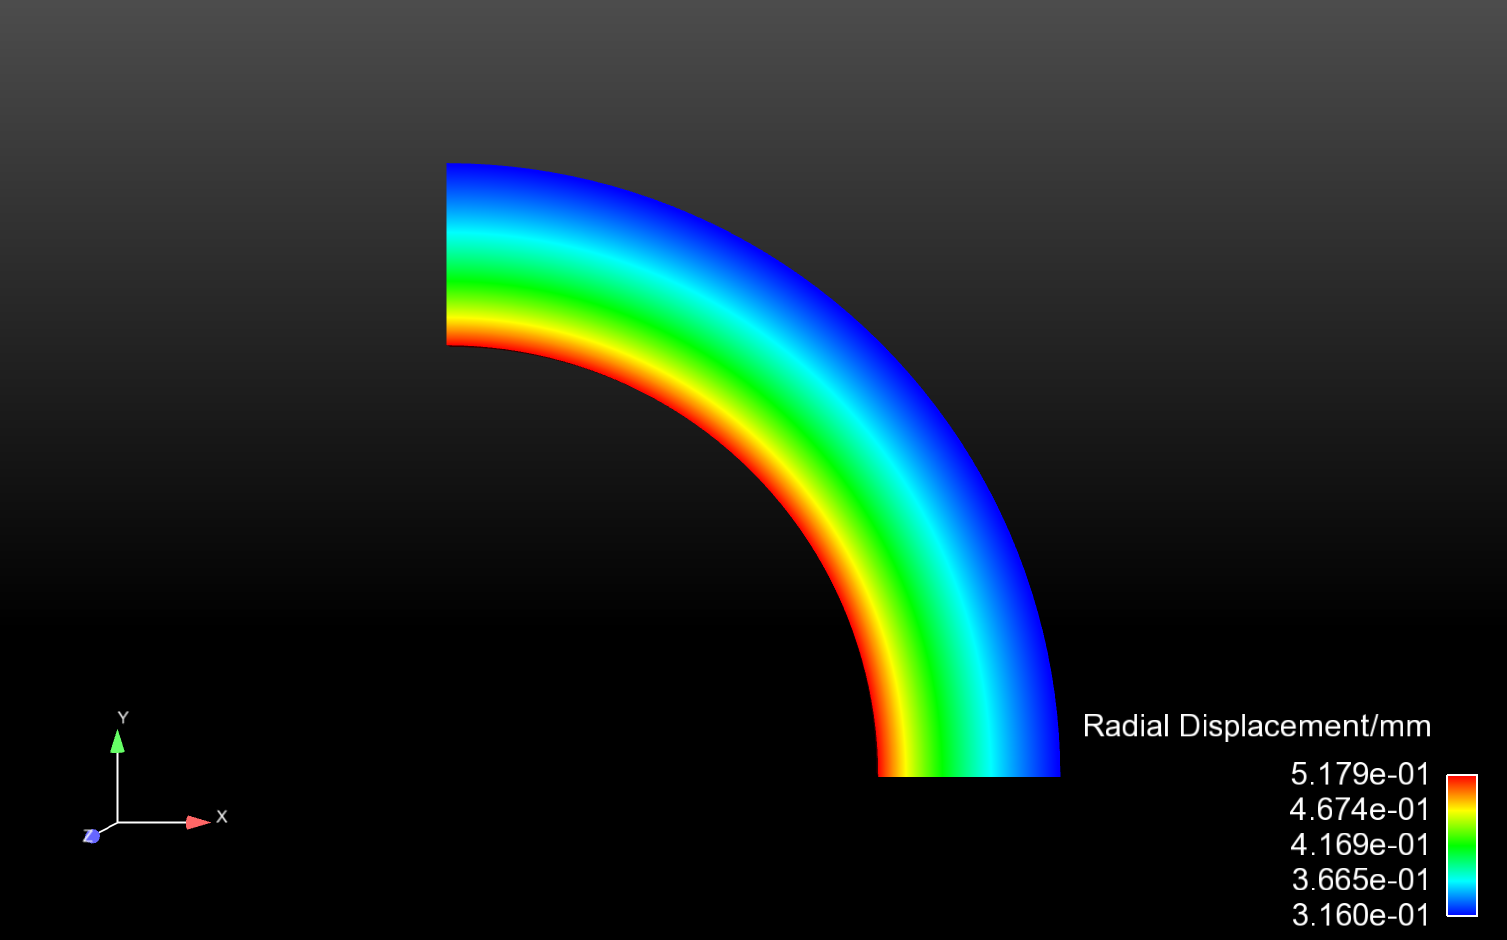
\includegraphics[width=\textwidth]{./figures/artery_ur.png}
		\caption{Radial displacement}
		\label{ur_artery}
	\end{subfigure}
	\begin{subfigure}[b]{0.5\textwidth}
		\centering
		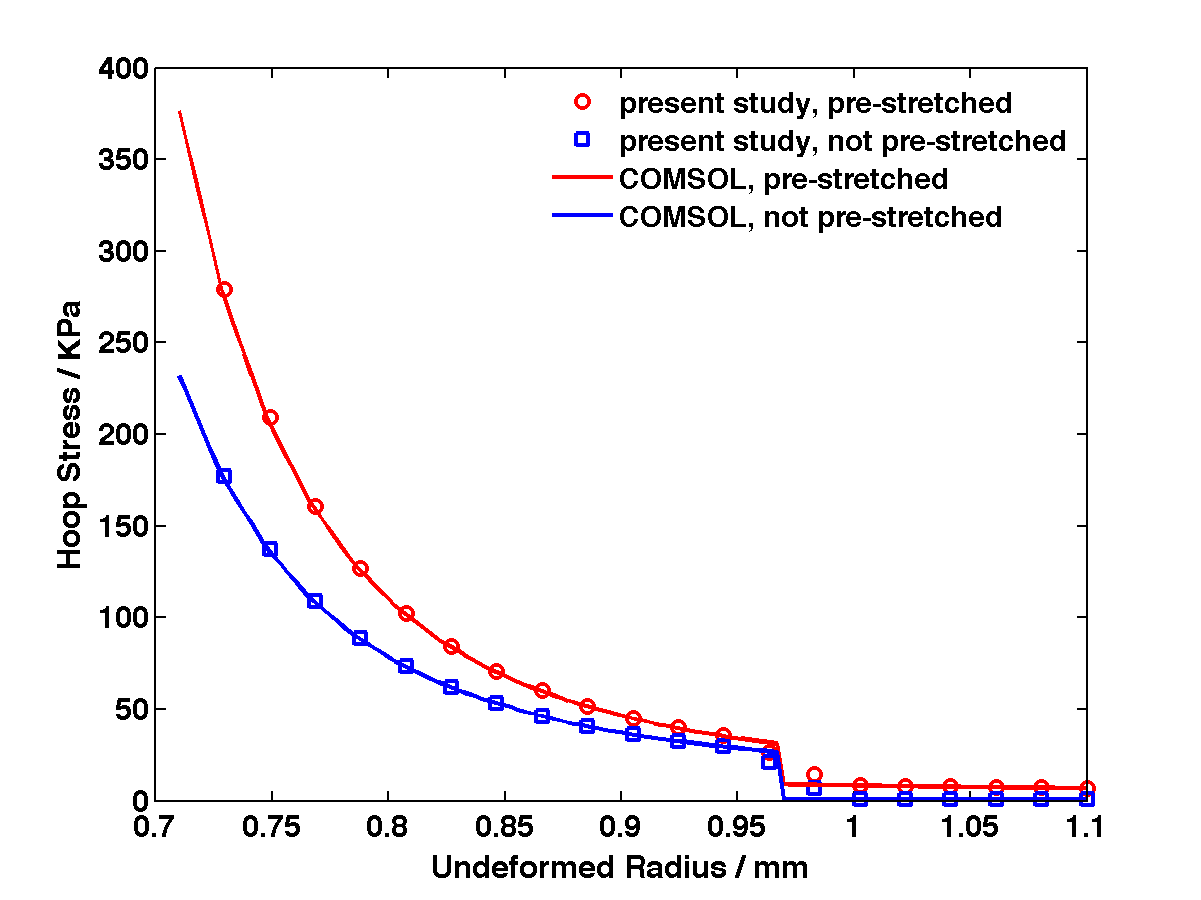
\includegraphics[width=\textwidth]{./figures/artery_hoop.png}
		\caption{Hoop stress}
		\label{hoop_artery}
	\end{subfigure}
	
	\begin{subfigure}[b]{0.5\textwidth}
		\centering
		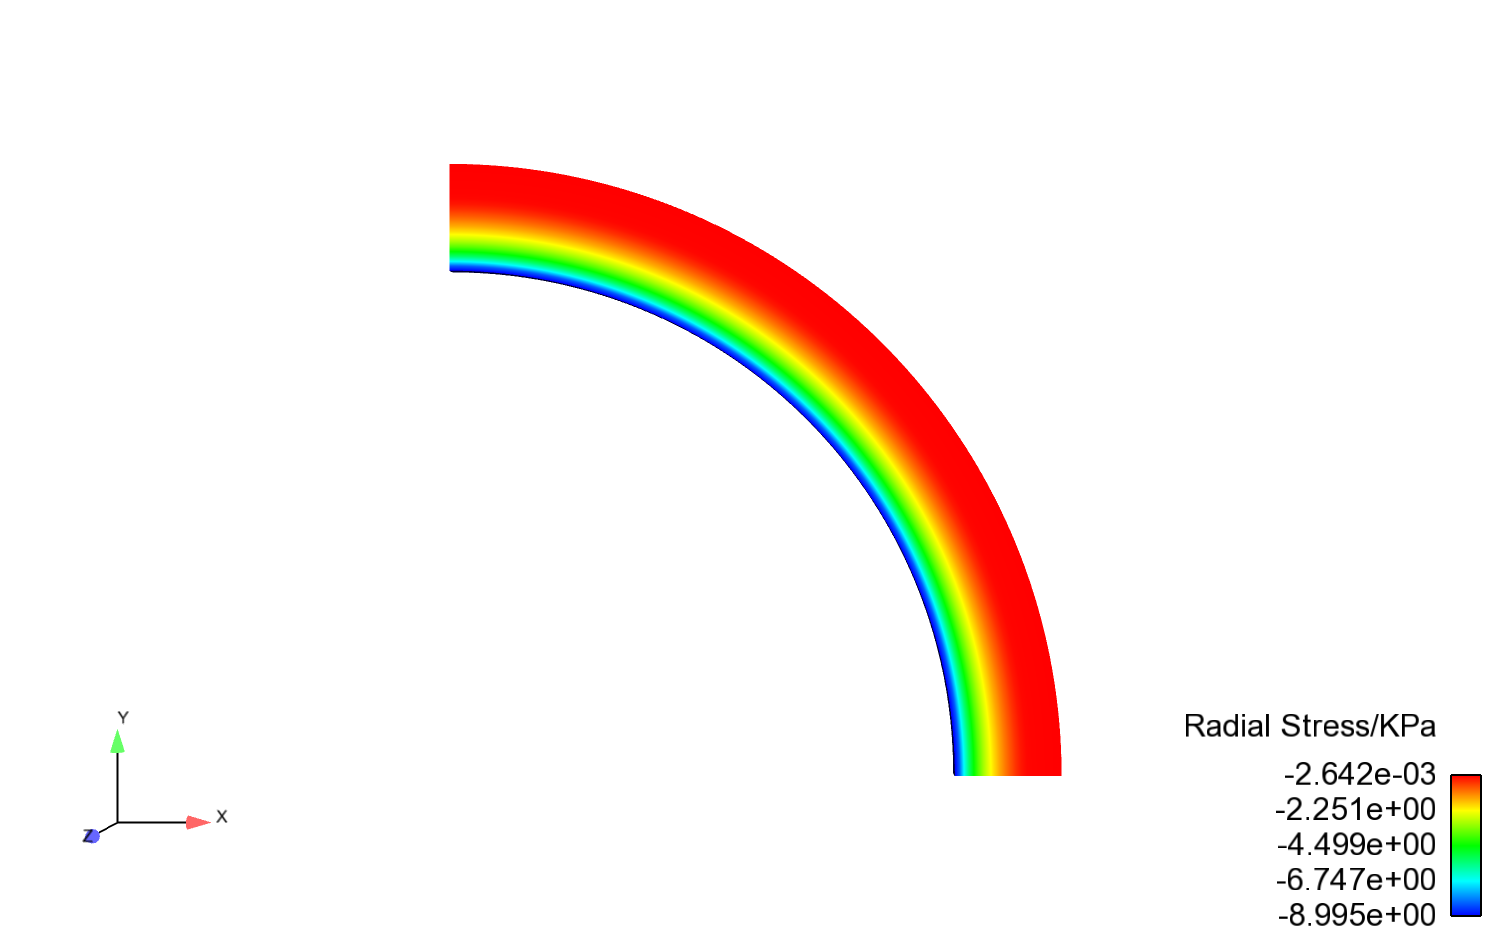
\includegraphics[width=\textwidth]{./figures/artery_radial.png}
		\caption{Radial stress}
		\label{radial_artery}
	\end{subfigure}
	\begin{subfigure}[b]{0.5\textwidth}
		\centering
		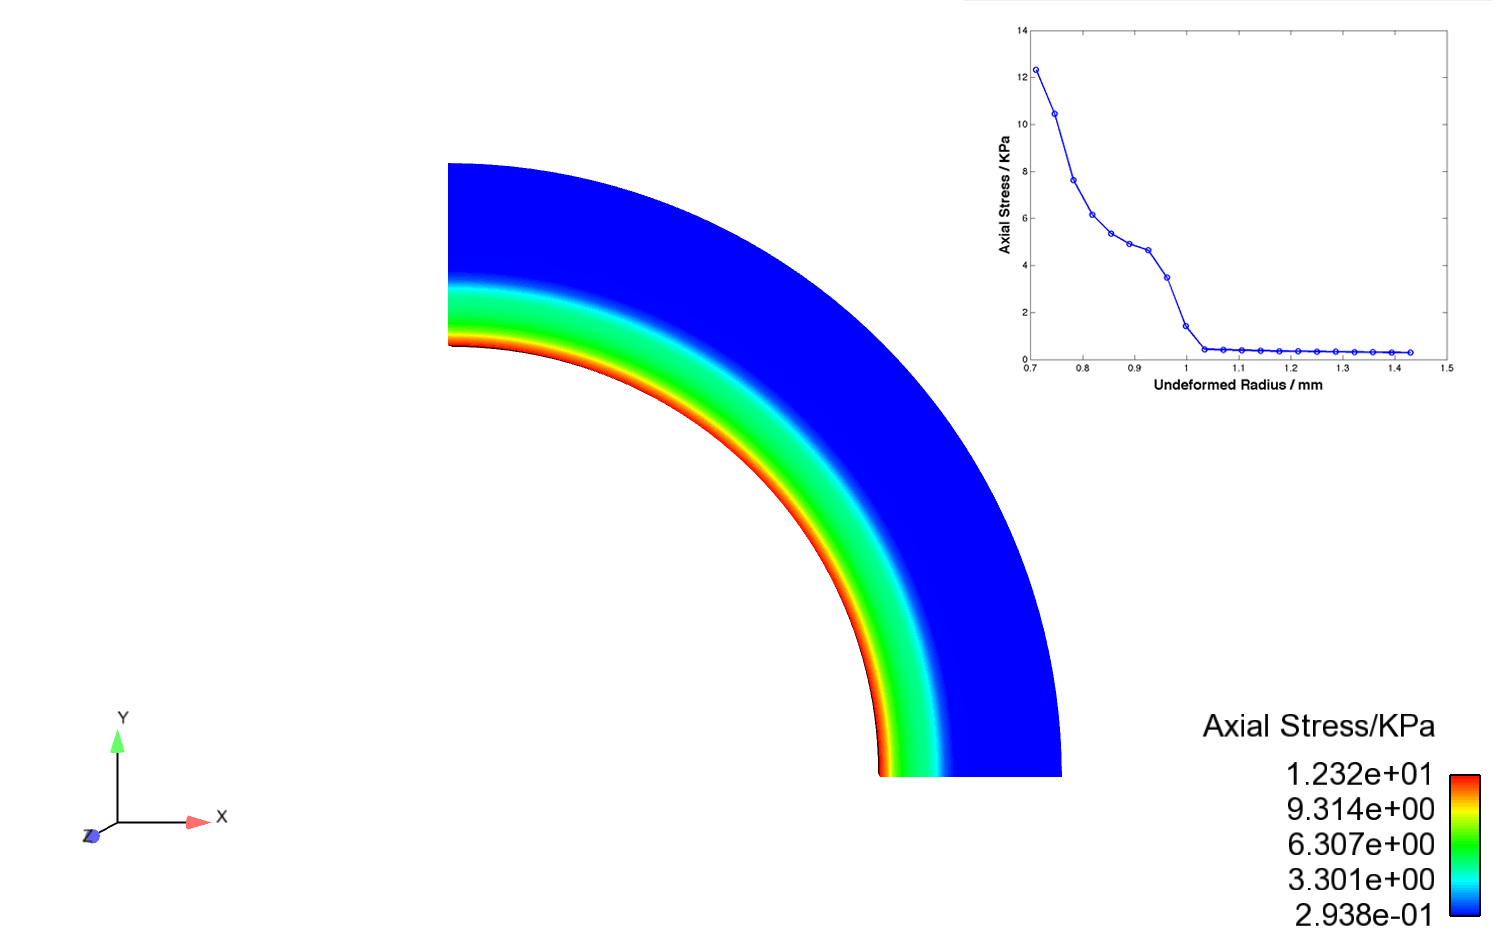
\includegraphics[width=\textwidth]{./figures/artery_axial.png}
		\caption{Axial stress}
		\label{axial_artery}
	\end{subfigure}
	\caption{Rabbit carotid artery under $10$ KPa}
	\label{fig:artery}
\end{figure}

















